\begin{figure}[t]
  \centering
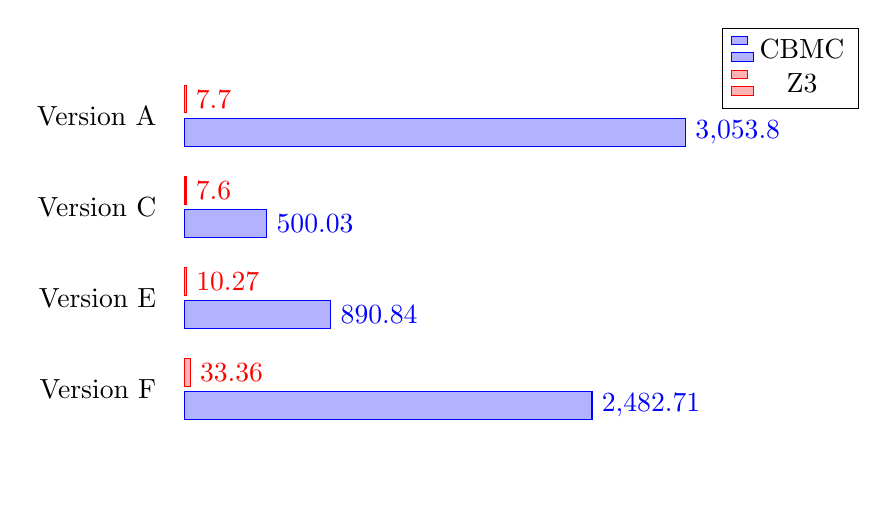
\begin{tikzpicture}
  \begin{axis}[
    xbar,
    y axis line style = { opacity = 0 },
    axis x line       = none,
    tickwidth         = 0pt,
    enlarge y limits  = 0.32,
    enlarge x limits  = 0.04,
    symbolic y coords = {Version F, Version E, Version C, Version A},
    nodes near coords,
    legend pos=outer north east,
  ]
  \legend{CBMC, Z3}
  \addplot coordinates { (3053.8,Version A)         (500.03,Version C)
                         (890.84,Version E)  (2482.71,Version F) };
  \addplot coordinates { (7.7,Version A)         (7.60,Version C)
                         (10.27,Version E)   (33.36,Version F)  };  
  \end{axis}
\end{tikzpicture}  
  \caption{CBMC Vs Z3 encoding for N $\equal$ 5 (in secs)}
  \label{fig:cz-comp}
\end{figure}

%%% Local Variables:
%%% mode: latex
%%% TeX-master: "main"
%%% End:
